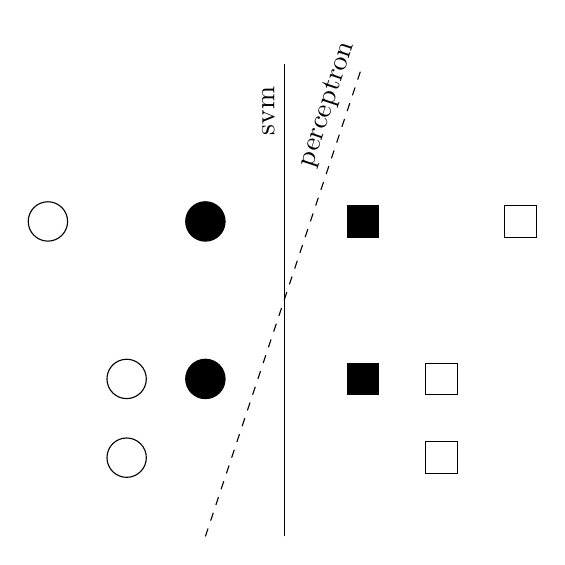
\begin{tikzpicture}

% \draw (-8, -5) grid (5, 5);

\draw [fill] (-1,1) circle (.25);
\draw [fill] (-1,-1) circle (.25);
\draw (-2,-1) circle (.25);
\draw (-2,-2) circle (.25);
\draw (-3,1) circle (.25);

\draw [fill] (1,1) ++(-.2,-.2) rectangle ++(.4,.4);
\draw [fill] (1,-1) ++(-.2,-.2) rectangle ++(.4,.4);
\draw (2,-1) ++(-.2,-.2) rectangle ++(.4,.4);
\draw (2,-2) ++(-.2,-.2) rectangle ++(.4,.4);
\draw (3,1) ++(-.2,-.2) rectangle ++(.4,.4);

\draw [dashed] (-1,-3) -- (1,3)
 node[pos=.9,sloped,above]{perceptron};
\draw (0,-3) -- (0,3)
 node[pos=.9,sloped,above]{\acs{svm}};

% \draw (-5,-2) circle (.125);
% \draw (-5,-1) circle (.125);
% \draw (-6,-1) circle (.125);
% \draw (-6,-2) circle (.125);
% \draw (-7,-2) circle (.125);

% \draw (-6.5,-1.3) ++(-.1,-.1) rectangle ++(.2,.2);
% \draw (-6,0) ++(-.1,-.1) rectangle ++(.2,.2);
% \draw (-6.7,-3) ++(-.1,-.1) rectangle ++(.2,.2);
% \draw (-5.5,-3.4) ++(-.1,-.1) rectangle ++(.2,.2);
% \draw (-4.7,-2.1) ++(-.1,-.1) rectangle ++(.2,.2);

% \draw [->, ultra thick] (-4.5, -2.5) -- (-2, 0)
%   node [pos=.5, sloped, above] {mappa $\Phi$};

\end{tikzpicture}